\chapter{Introduction}

\begin{figure}
	\centering
	\begin{subfigure}{0.45\textwidth}
		\centering
		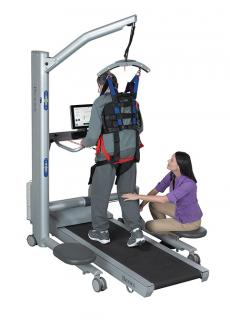
\includegraphics[height=3in]{gait_training.jpg} % first figure itself
		\caption{Conventional gait rehabilitation. \cite{gaitrehabgantry}}\label{fig:gantry}
	\end{subfigure}\hfill
	\begin{subfigure}{0.45\textwidth}
		\centering
		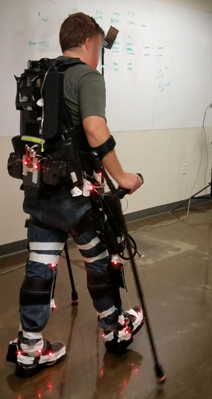
\includegraphics[height=3in]{subject.png}
		\caption{EksoGT - powered exoskeleton}\label{fig:subject}
	\end{subfigure}
	\caption{Methods of gait rehabilitation}
\end{figure}

\section{Motivation}
%
%\begin{figure}
%	\centering
%	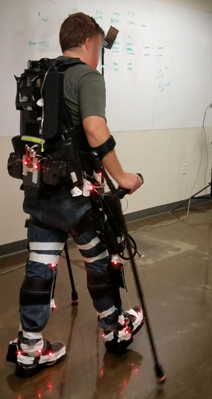
\includegraphics[width=0.15\linewidth]{subject.png}
%\end{figure}

\textit{Better opener than the quarter million line}. In addition to an adverse impact on the quality of life, cost of care per patient with Spinal Cord Injuries (SCIs) exceeds half a million dollars \cite{devivo2011costs}. One of the main mechanisms of recovery from SCIs is the reorganization of the patient's intact neuronal pathways \cite{curt2008recovery}. In order to take advantage of this neural plasticity, gait rehabilitation strategies involve repeatedly moving the patient's legs through prescribed walking trajectories. Conventionally, this process involves physiotherapists manually moving the patient's legs to track the desired trajectories (Fig.~\ref{fig:gantry}). The main drawback of this approach is that the necessary joint trajectories may not be tracked accurately as the treatment progresses due to therapist exhaustion. Robotic exoskeletons have recently come into use for rehabilitation due to their ability to consistently track the desired trajectories, which may accelerate recovery \cite{hidler2011role}. Multiple exoskeletons, such as the Ekso GT \cite{brenner2016exploring} (Fig.~\ref{fig:subject}), Indego \cite{sup2008design}, and ReWalk \cite{rewalk}, have been cleared by the FDA for use in gait rehabilitation. Physiotherapists may act in a supervisory role instead of actively guiding the patient's legs through the desired trajectories due to the application of exoskeleton to gait rehabilitation. 

Exoskeleton usage increase the patient's level of autonomy and fluent Human-Robot Interaction (HRI) is desired to maintain the safety and efficacy of the treatment. While an abstract notion, fluency in HRI can be roughly defined as the reliability with which a human and robot can predict each other's actions~\cite{hoffman2007cost}. In addition to device safety, increasing fluency will help the user locomote more naturally and reduce the cognitive load on the user caused by using the device. Gait patterns have been shown to be affected by cognitive load \cite{bogen2018walk} so reducing it may yield more natural gait patterns. It may be quantified by the inverse of the time it takes to complete desired tasks \cite{hoffman2019evaluating}. Fluency in HRI can be increased if the robot can anticipate the user's intent and assist accordingly. The overall goal of this work is to estimate user intent to increase the fluency of lower-extremity exoskeletons. Intent itself is difficult to quantify, so a user's desired forward velocity is considered as an expression of intent. Model-based and data-driven methods are considered to infer user intent by studying the effects of changes in velocity on gait patterns.

\section{Fluency of HRI through accurate intent estimation}

A robot's ability to deliver timely assistance to the user is an important indicator of fluency. Anticipative intent estimation methods are necessary to reduce the delay in robot assistance delivery after the user has changed their intent. These methods estimate intent changes before they are physically realized, in contrast to reactive methods that detect changes after realization. Intent estimation should ideally be anticipative than reactive as the timing of the assistance is crucial for fluent HRI. Control actions necessary for assistance delivery may be decided in advance of when they need to be executed and assistance may be delivered more precisely due to anticipative intent inference. Therefore, anticipative intent estimation is important for high fluency in HRI.

\begin{figure}
	\centering
	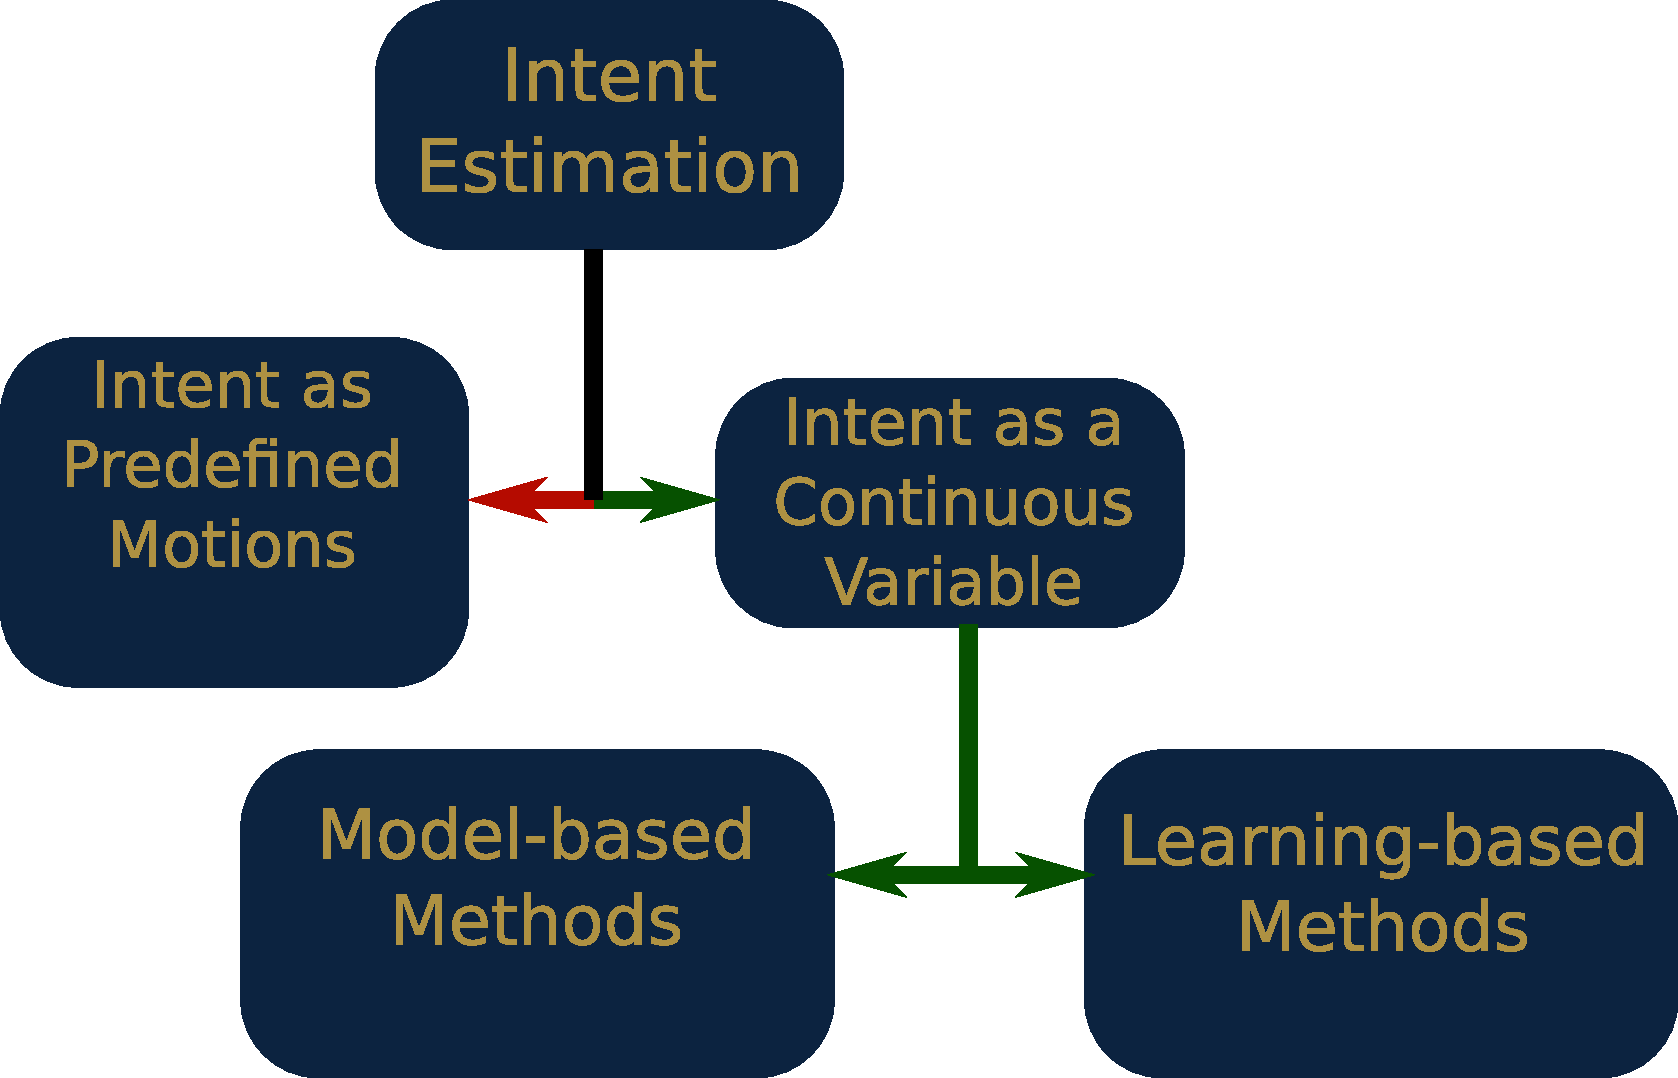
\includegraphics[width=0.7\linewidth]{intent_flow_chart.pdf}
	\caption{Possible approaches to intent estimation. Approaches considered in this work have been indicated with green arrows.}\label{fig:flow}
\end{figure}

HRI itself can be used to estimate user intent. As illustrated in Fig.~\ref{fig:flow}, one approach is to infer intent posed as a discrete variable and infer it by comparing measurements of user activity to a database of predefined activities such as sitting, standing, steady-state walking, and the transitions between them \cite{shen2013motion}. Generating databases containing a wide range of such activities may be prohibitive. Alternatively, intent may be treated as a continuous state to achieve finer control of the assistive device. User intent estimation may be performed by leverage the HRI in gait rehabilitation. One study used physical Human Robot Interaction (pHRI) to estimate the user intent in collaborative reaching motions  \cite{corteville2007human}. In it, the human was considered to be in control of the HRI and measurements of the user's motion acquired using sensors onboard the robot were fit to a velocity profile to estimate the intended speed of the movement. 

Another approach to use pHRI for user intent estimation is to compare the user's efforts to the total effort necessary to accomplish the desired task \cite{pehlivan2015minimal}. The human-robot system's interaction with the environment may also be considered pHRI and may be used to estimate user intent. For example, Inertial Measurement Units (IMUs) were mounted to crutches to estimate their orientation \cite{brescianini2011ins}. This allowed the inference of user intent variables such as stride length, direction, stair ascent/descent based on crutch placement. The reliance of many state-of-the-art approaches on sensors like EMGs, electrogoniometers, IMUs, force sensors may be problematic in practical applications as EMG sensors need consistency in placement any may slip during usage due to perspiration \cite{tkach2010study,ison2014role}. Therefore, relying on sensors onboard the exoskeleton may offer a more reliable option \cite{Gambon20b}. 

While pHRI may be used to infer an exoskeleton user's intent, the presence of injuries and their severity may limit the extent to which pHRI may be leveraged. HRI has been used to great effect in assisting healthy individuals walking in hip exoskeletons by modeling the impedance of the coupled human-robot system \cite{zhang2019admittance,nagarajan2016integral}. Hip torques generated by the user govern the assistance provided by the exoskeleton. However, it may be difficult to adapt these strategies to individuals with iSCIs due to significant lower-limb impairment. Some available exoskeletons that are targeted toward individuals with iSCIs use rudimentary methods to infer user intent. The HAL exoskeleton uses force sensors under the feet to detect weight transfer to initiate a step \cite{suzuki2007intention} and the ReWalk system uses a combination of ground reaction force sensors and torso tilt \cite{goffer2012locomotion}. While these intent detection strategies leverage basic pHRI, incorporating variables such as stride information in intent estimation that may provide additional insight into the user's desired motion through their gait patterns using model- or learning-based strategies, proceeding to the third level of Fig.~\ref{fig:flow}.

\section{Model-based and learning-based approaches to estimation}

Mechanically, humans are high degree of freedom systems but their gait patterns can often be accurately described by reduced order models. Human walking can be modeled using template models and anchor models~\cite{full1999templates}. Template models are reduced order models that emulate the salient characteristics of locomotion and abstract the complexities of neuro-muscular interaction. Anchor models are higher fidelity models based on human morphology that combine template models with human physiology. The additional complexities found in anchor models make computational tasks such as estimation and control based on anchor models more computationally intensive, rendering them inappropriate for use in online processes such as intent detection. While detailed musculo-skeletal models offer subject-specific insight into walking, the omission of these complexities in template models make them more suited for general use across subjects. This generality and reduced order makes template models more suited for use in control and estimation problems for legged locomotion.

Template models often use parameters such as center of mass (CoM) height, velocity, and leg stiffness to describe gait. It may be possible to estimate and exoskeleton user's intended forward velocity by comparing measurements of these parameters with gaits simulated using models of locomotion. For example, intent estimation in lower-extremity exoskeletons based on orbital energy \cite{chen2018dynamic} has been carried out using the Linear Inverted Pendulum (LIP) model, which is a simple model of legged locomotion.  Alternatively, data-driven estimation strategies \cite{ge2011neural, kalinowska2019data, joukov2017rhythmic} may be used to handle gait characteristics that may be difficult to model using physics-based models.

Learning-based strategies use gait data to form relationships between sensor measurements and gait features such as foot placement and step frequency. Convolutional Neural Networks (CNNs) \cite{lee2020image}, decision trees \cite{moolchandani2021design}, and Linear Discriminant Analysis (LDA) \cite{young2013classifying}  have all been used to estimate human intent in real-time with low error rates using sensors such as potentiometers and encoders onboard the prosthesis \cite{young2013classifying}, electrogoniometers \cite{lee2020image}, and force plates \cite{moolchandani2021design} in addition to  electromyography (EMG) and IMUs. A Gaussian Process (GP) based Extended Kalman Filter has been used to estimate a user's gait phase during stance to control a powered prosthetic leg \cite{thatte2019robust}. This work is targeted toward individuals with iSCIs whose gait patterns depend the severity of the injury \cite{rota2011walk}. Therefore, subjects' interactions with the robot and the environment may show individualized trends making estimator personalization necessary for intent change estimation from gait patterns. 

\section{Personalizing intent estimation and addressing data scarcity}

Learning-based approaches for intent estimation often rely on large amounts of data to generate models gait features. Acquiring this data for injured population is made increasingly difficult due to changes in gait patterns due to severity of injuries \cite{sohn2018variability}. The difference in gait patterns across individuals makes estimator personalization unavoidable. Acquiring adequate amounts of data to train a single model to perform estimation across multiple individuals is difficult as gait variability resulting from spasticity due to iSCIs \cite{krawetz1996gait} needs to be accommodated. Data scarcity may be addressed by combining training data from multiple subjects.

There is underlying commonality, across individuals, in changes to gait patterns relating to changes in gait velocity. For example, step length and frequency, pitch and roll motions of the torso, and joint trajectories all show qualitatively similar trends relating to changes in the desired gait velocity across individuals. Training data scarcity may be addressed by exploiting this commonality to personalize intent estimation by transforming easily accessible gait data from healthy individuals using a small amount of user-specific data.

\section{Contributions and organization}

Robotic exoskeletons such as the EksoGT, ReWalk and Indego have been approved by the FDA for gait rehabilitation of individuals with iSCIs, yet they lack high fluidity in HRI. The intent change estimation in these devices is reactive and limited to detecting when the user wants to initiate a new step of a predifined gait pattern. This limitation also prevents sudden velocity changes. As a result, these devices are generally seen in clinical settings and their operation requires physiotherapist supervision. Increasing the HRI fluency in these devices may make unsupervised use of these devices possible which may lead to increased usage and accelerated rehabilitation \cite{hidler2011role}. This dissertation makes three contributions with n aim to advance the state-of-the art of intent estimation to be more anticipative of changes in the user's intent as expressed through gait velocity and increase the fluency in HRI.

\begin{itemize}
	%\item \textbf{Contribution 1: Model-based Approach to Estimate Gait Characteristics:} 
	\item Accurate state estimation is a foundational component for intuitive user intent detection in HRI, as it would deliver increased insight into user actions. The first contribution was to establish a framework capable of handling hybrid dynamics to estimate gait characteristics such as gait phase, using simulated gaits of physics-based models of legged locomotion (Chapter~\ref{chapter:IMM}).
	%\item \textbf{Contribution 2: Intent Change Estimation Based on Physical Interactions of an Exoskeleton User:} 
	\item In contrast to many state-of-the-art intent estimators that are reactive, this objective is to develop an estimator that anticipates changes in the exoskeleton user’s intended gait velocity by analyzing how the user interacts with the robot and the environment to realize the desired change. This estimator was evaluated with walking trial data of	individuals with and without iSCIs walking in an EksoGT exoskeleton. The differences in the interactions of injured and uninjured users was explored (Chapter~\ref{chapter:BKF}).
	%\item \textbf{Contribution 3: Personalization of Estimation in the Presence of Data Scarcity:}
	\item The inter-subject gait variability observed across individuals motivated personalizing estimation of changes in intended gait velocity of exoskeleton users. One of the main hurdles in achieving the required personalization is the scarcity of user-specific training data due to difficulty in acquisition. Estimator personalization was achieved by exploiting commonalities in gait patterns across users and augmenting base data from healthy subjects with user-specific data from subjects with injuries (Chapter~\ref{chapter:MP}).
\end{itemize}